\documentclass[]{scrartcl}
\title{Vorlesung Analysis II}
\usepackage{amsmath,amssymb,amsfonts}
\usepackage{stmaryrd}
\usepackage{mathtools}
\usepackage{latexsym}
\usepackage{graphicx}
\usepackage{tikz}
\usepackage{xcolor}
\usepackage{soul}
\usepackage{hyperref}
\usepackage{tipa}
\usepackage[dvipsnames]{xcolor}
\hypersetup{
	colorlinks=true,
	linkcolor=blue,
	filecolor=magenta,      
	urlcolor=cyan,
	pdftitle={Overleaf Example},
	pdfpagemode=FullScreen,
}
\newcommand{\redcircle}[1]{%
	\tikz[baseline=(char.base)]{
		\node[shape=circle, draw=red, text=red, thick, inner sep=1pt] (char) 
		{\textbf{#1}};
	}%
}
\setul{1pt}{1.5pt} % Linienhöhe und Abstand zum Text (optional anpassbar)

\setlength{\topmargin}{-.5in} \setlength{\textheight}{9.25in}
\setlength{\oddsidemargin}{0in} \setlength{\textwidth}{6.8in}
\setlength{\parindent}{0pt}

\begin{document}
	\maketitle
	\textbf{\underline{an3: Konvergenz, Funktionsgrenzwerte, Stetigkeit im 
	$\mathbb{R}^n$}}\\
	\\
	\textbf{\underline{\underline{Stichwörter:}Funktionsgrenzwerte, Stetigkeit 
	( Komponentenweise und partiell)}} \\
	\\
	\textbf{\underline{Literatur:}}\setulcolor{blue}\ul{[Hoff], Kapitel 9.3}\\
	\\
	\textbf{3.1\underline{Einleitung:}} Wir definieren Funktionsgrenzwerte bei Funktionen f von $\mathbb{R}^n$ nach $\mathbb{R}^m$\\
	\\
	\textbf{3.2 \underline{Vereinbarung/Situation:}} Seien M,n $\in \mathbb{N}$, M $\subseteq \mathbb{R}^n$, f : D $\rightarrow \mathbb{R}^m$ \\
	und b $\in \mathbb{R}^m$. Als Norm benutzen wir die \setulcolor{Orchid}\ul{Maximumsnorm} und schreiben deswegen $||\cdot||$ für $||\cdot||_\infty$. Weiter sei $a \in \mathbb{R}^n$ ein Häufungspunkt zu/von M, d.h $\forall \epsilon > 0 : \neq $\setulcolor{red}\ul{$\{x\in M; ||x-a||<\epsilon\}$} 
	= $\infty$ (vgl. \setulcolor{blue}\ul{An 10.2}).\\
	(Anmerkung\ul{$\{x\in M; ||x-a||<\epsilon\}$} = \setulcolor{yellow}\ul{$U^\epsilon_a(M)$}$\leftarrow$\setulcolor{red} \ul{$\epsilon$-Umgebung} um a, vgl. \setulcolor{blue}\ul{3.14}).\\
	Dies bedeutet, dass a aus M heraus durch von a verschiedene Punkte x $\in M$ beliebig gut approximierbar ist, bzw. "man kommt mit Punkten aus M beliebig gut heran an a", und zwar aus "allen Richtungen" falls $\exists \epsilon > 0 : U^\epsilon_a(\mathbb{R}^n)\subseteq M$.\\
	Wie in \ul{An 10.4} definieren wir dann den Funktionsgrenzwert:
	\\\\
		
	\textbf{3.3\underline{Def.:}} In Situation \ul{3.2} gilt: f(x) $\rightarrow$ b (für M$\ni$ x $\rightarrow$ a)\\
	: \setulcolor{red}\ul{$ \Leftrightarrow\forall \epsilon > 0 \exists \delta 
	> 0$ \hspace{5mm} $ \forall x \in M: 0\textless||x-a|| < \delta  
	\Rightarrow || f(x) - b || < \epsilon$}\\
	Lesen: "f(x) Konvergiert gegen b, wenn x (aus M heraus) gegen a 
	geht/Konvergiert".\\
	Wir nennen b $\in \mathbb{R}^m$ den  \ul{Grenzwert} (Kurz \ul{GW})\ul{von f(x) für $M \ni x \rightarrow a.$}\\
	Notation: f(x) $\xrightarrow[]{M\ni x \rightarrow a}$b oder $\lim_{M \ni x 
	\rightarrow a} f(x)=b$ oder $\lim\limits_{x\rightarrow a|x\in M}f(x)=b.$\\
	Umformulierung:$||f(x)-b||\xrightarrow{M\ni x\rightarrow a}0.$\\\\
	
	\textbf{3.4\underline{Bem.:}} Falls M = D ist, hat die Bedingung "$x\in M$" Keine Weitere Bedeutung und kann weggelassen werden. Fehlt eine Bedingung, ist einfach m= D gemeint.\\\\
	
	\textbf{3.5}Funktionsgrenzwerte können \underline{Komponentenweise} untersucht und gebildet werden:\\
	Für $ x \in D$ ist f(x) ein Element des $\mathbb{R}^m$, also Schreibbar in den Komponenten/Koordinaten\\
	f(x)=$\begin{pmatrix}
		f_1(x)\\f_2(x)\\\vdots\\ f_m(x)
	\end{pmatrix}$, den Komponentenfunktionen $f_1,...,f_m: D\rightarrow\mathbb{R}$, nämlich $\forall i \in \{1,...,m\}:$ \setulcolor{red} \ul{$f_i:=pr_i\circ f$}.\\
	Mit $b= (b_1,...,b_m)^T \in \mathbb{R}^m$ gilt dann:\\
	\textbf{\underline{Beh.:}} \begin{equation}\begin{split}
		f(x)\xrightarrow{M\ni x \rightarrow a}b & \Leftrightarrow \forall i \in 
		\{1,...,m\}: f_i (x)\rightarrow b_i (M\ni x\rightarrow a)\\
		 & \Leftrightarrow\forall i: |f_i(x)-b_i|\rightarrow0(M\ni x 
		 \rightarrow a)
		\end{split}
	\end{equation} 
	\textbf{\underline{Bew.:}} Für $z= (z_1,...,z_m)^T \in \mathbb{R}^m, i\in \{1,...,m\}$ gilt $|z_i-b_i|\leq||z-b||_\infty \leq \sum_{i=1}^{m}|z_i-b_i|.$\\
	\strut\hfill $\square$\\
	\textbf{3.6\underline{Bem.:}} Mit \setulcolor{blue} \ul{3.5} kann man sich also auf die kgz. der Komponentenfunktionen zurückziehen , falls das nützlich/schneller geht.\\
	\textbf{3.7\underline{Bsp.:}} $D = \mathbb{R}^2 \backslash\{\begin{pmatrix}0\\0\end{pmatrix}\}, f(v):=\frac{xy}{\sqrt{x^2+y^2}}$, wenn $v=\begin{pmatrix}x\\y\end{pmatrix} \in D$, also $f:D\rightarrow\mathbb{R}$.\\
	\underline{Beh.:} $f(v)\rightarrow0$ (bei $D \ni v \rightarrow(0,0)^T=:0$).\\
	\underline{Bew.:} $|f(v)-0| = |f(v)| \leq \frac{||v||^2_2}{||v||_2}= ||v||_2\rightarrow0.$\\
	Bei  $\leq \frac{||v||^2_2}{||v||_2} \Leftarrow |xy|\leq $max$(x^2,y^2)=||v||^2\leq x^2+y^2=||v||^2_2$.\\
	\strut\hfill$\square$\\
	\textbf{3.8\underline{Bsp.:}} $D = \mathbb{R}^2 
	\backslash\{\begin{pmatrix}0\\0\end{pmatrix}\}, 
	f(v):=\frac{xy}{x^2+y^2}$, wenn $v=\begin{pmatrix}x\\y\end{pmatrix} 
	\in D$, also $f:D\rightarrow\mathbb{R}$.\\
	\underline{Beh.:} Es existiert kein $b\in \mathbb{R}$ mit $f(v)\rightarrow
	b$ (bei $v\rightarrow (0,0)^T=0$).\\
	\underline{Bew.:} Für x$\in \mathbb{R}\backslash\{0\}$ gelten $f(x,0)=0$ 
	und $f(x,x)=\frac{1}{2}$, im $\lightning$ zu \setulcolor{blue} \ul{3.5.}\\
	\strut\hfill$\square$\\
	Wie in eindimensionalen Fall ist ein Funktions GW mit Folgenkonvergenz 
	beschreibbar:\\
	\textbf{3.9 \underline{Bem.:}}  $f(x) \xrightarrow{M\ni x\rightarrow a}b$, 
	wenn $\forall (x_k)_{k\in \mathbb{N}} \subseteq M, x_k 
	\xrightarrow{k\rightarrow \infty}a: f(x_k)\xrightarrow{k\rightarrow 
	\infty}b$ mit Folgenkonvergenz wie in \ul{an 1.8}\\
	\\
	\textbf{3.10 \underline{Rechnen mit Grenzewerten} 
	\setulcolor{red}("\ul{GWSätze}")}:\\

	\begin{align}
		f(x)\rightarrow b, g(x)\rightarrow c & \Rightarrow 
		(f+g)(x)\rightarrow b \pm c\text{, sofern bildbar}\\
		& \Rightarrow \textless f(x), g(x)\textgreater\rightarrow\textless 
		b,c\textgreater\text{, sofern bildbar}\\
		& \Rightarrow ||f(x)|| \rightarrow ||b||
	\end{align}
\\
	Wir kommen zur Stetigkeit von Funktionen $f:D\rightarrow\mathbb{R}^m, 
	D\subseteq\mathbb{R}^n.$\\
	\textbf{3.11\underline{Def.:}}\setulcolor{red}\\
	\begin{align}
		\text{Für }a\in D \text{ heißt f \ul{stetig in a} :} &\Leftrightarrow 
		\forall \epsilon\textgreater0 \exists \delta \textgreater 0 \forall x 
		\in D:||x-a||\textless \delta \Rightarrow ||f(x)-f(a)|| 
		\textless\epsilon\\
		& \Leftrightarrow f(x)\rightarrow f(a) (\text{bei } D\ni x \rightarrow 
		a)\\
		&\text{bzw. }\lim_{x\rightarrow a (x \in D)} f(x)= f(a).
	\end{align}
	\\
	\textbf{3.12 \underline{Bem.:}} Die Forderung, dass a ein Häufungspunkt von 
	D ist, wird hier nicht benötigt.\\
	\textbf{3.13 \underline{Def.:}} Sei $T\subseteq D$. Dann: f heißt \ul{setig 
	in T} $:\Leftrightarrow \forall z \in T: f$ stetig in z\\
	f heißt \ul{Stetig} $:\Leftrightarrow f$ stitig in D\\
	\\
	\textbf{3.14} Zum Erkennen von stetigen Funktionen ist wieder folgende 
	Grundregel zur Stetigkeit zusammengesetzter/verknüpfter Funktionen 
	nützlich:\\
	\underline{Vor.:} $n,m,k\in \mathbb{N},\ a \in D\subseteq \mathbb{R}^n,\ 
	f:D_1\rightarrow\mathbb{R}^k,\\
	D_1 \subseteq\mathbb{R}^m$ mit $f(D)\subseteq D_1,\ 
	h:D_1\rightarrow\mathbb{R}^k,\\
	b:=f(a), f$ in a stetig, h in b stetig.\\
	\underline{Beh.:}\setulcolor{green}\ul{$h\circ f: D\rightarrow 
	\mathbb{R}^k$ ist in a stetig}\\
	\underline{Skizze:}\\
	\begin{figure}[h]
		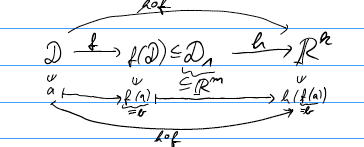
\includegraphics[width=7 cm,height=3cm]{skizze kap 3}
	\end{figure}\\
	\underline{Bezeichnung:} \setulcolor{yellow} 
	\ul{$U^S_c$}:=\setulcolor{red}\ul{$\{x\in \mathbb{R}^l; ||x-c||\textless 
	S\}$} heißt \ul{S-Umgebung von c} Bedeutung der Stetigkeit von $h\circ f:$ 
	eine $\eta$-Umgebung von a wird unter f in eine $\delta$-umgebung von b, 
	und diese dann unter h ist eine $\epsilon$-Umgebung von h(b) abgebildet. 
	Dies ist auch der\\
	\underline{Bew.:}\\
	Zu $\epsilon\textgreater 0$ ex. zunächst ein $\delta \textgreater 0$ so, 
	dass $||h(z)-h(b)|| \textless \epsilon$ (bei $z \in D_1, ||z-b|| \textless 
	\delta$).\\
	Zu $\delta\textgreater 0$ ex. nun ein $\eta \textgreater 0$ so, dass 
	$||f(x)-f(a)||\textless \delta\ (\text{bei } x\in D ,|| x-a||\textless 
	\eta).$\\
	Für solche x gilt also $||h(f(x))-h(f(a))||\textless \epsilon$. Also ist h 
	$\circ$ f stetig in a.\\
	\strut\hfill$\square$\\
	\textbf{3.15 \underline{Beh.:}}\setulcolor{blue}\ul{3.5} liefert nun mit  
	\ul{3.14}, dass Stetigkeit und Komponentenweise Stetigkeit (d.h. mit den 
	Komponentenfunktionen) äquivalent sind:\\
	\underline{Beh.:} \setulcolor{green}\ul{f stetig in a} $\Leftrightarrow$ 
	\ul{$\forall_i \in \{1,...,m\}:f_i$ stetig in a.} (Beachte $f_i=pr_i\circ 
	f$ und \setulcolor{blue}\ul{3.20})\\
	\underline{Bew.:} $"\Rightarrow"$: klar mit \ul{3.14/3.20} $"\Leftarrow"$: 
	Wähle $(x_k) \subseteq D$ mit $x_k\rightarrow a.$ Dann:\\
	$\forall i: pr_i(f(x_k))\rightarrow pr_i(f(a))$, da die $pr_i\circ f=f_i$ 
	stetig. Nach \ul{3.5} gilt dann $f(x_k)\rightarrow f(a)$, d.h. f ist stetig 
	in a laut \ul{3.11}.\\
	\strut\hfill$\square$\\
	Die GWSätze \ul{3.10} zeigen:\\
	\textbf{3.16 \underline{Kor.:}} Linearkombinationen stetiger Funktionen 
	(insbesondere Summen und Differenzen) und (soweit bildbar) Skalarprodukte 
	und Normen stetiger Funktionen sind wieder stetig.\\
	\\
	\textbf{3.17 \underline{Triviales Bsp.:}} $b\in\mathbb{R}^m$, die konstante 
	Fkt. f(x):= b für jedes $x\in\mathbb{R}^n$ ist stetig.\\
	\underline{Tivialität:} f stetig, $T\subseteq D\Rightarrow f r T$ stetig.\\
	\\
	\textbf{3.18 \underline{Satz:}} Jede \setulcolor{green} \ul{Lineare Abb.} 
	$A:\mathbb{R}^n\rightarrow\mathbb{R}^m$ ist \ul{stetig}. (im Sinne der 
	Lineare Algebra, s. \setulcolor{blue}\ul{Anhang 22 in an}1)\\
	\underline{Bew.:} Sei A durch die mxm-Matrix ($\alpha_{ij})_{1\leq i\leq 
	m|1\leq j\leq n}\in\mathbb{R}^{mxn}$ beschrieben, schreibe auch A für diese 
	Matrix. Für $x \in \mathbb{R}^n$ und $b:=Ax$ ist dann 
	$b_i=\sum_{j=1}^{n}\alpha_{ij}x_j$, wo $1\leq i \leq m$.\\
	Schätze ab: \setulcolor{orange}\ul{$|b_i|\leq 
	\sum_{j=1}^{n}|a_{ij}|\cdot|x_j|\leq 
	\sum_{j=1}^{n}|\alpha_{ij}|\cdot||x||,$} also \ul{$||Ax||\leq K\cdot||x||$}
	mit \ul{K:=$\max_{1\leq i\leq m}\sum_{j=1}^{n}|\alpha_{ij}|$.}\\
	Für $x,y\in\mathbb{R}^n$ gilt somit $||Ax-Ay||=||A(x-y)||\leq K\cdot 
	||x-y||,$ es folgt die Beh.\\
	\strut\hfill$\square$\\
	\textbf{3.19 \underline{Bsp.:}} $+:\mathbb{R}^2\rightarrow\mathbb{R}, 
	(x,y)\rightarrowtail x+y, \mathbb{R}^2\rightarrow\mathbb{R}, 
	(\alpha,x)\rightarrowtail \alpha\cdot x, 
	/:\mathbb{R}\backslash\{0\}\rightarrow\mathbb{R}, 
	x\rightarrowtail\frac{1}{x},$\\
	sind \setulcolor{green}\ul{stetige Abb.}.\\
	\\
	\textbf{3.20 \underline{Kor.:}} $\forall_i:$ 
	\ul{$pr_i$}:$\mathbb{R}^n\rightarrow\mathbb{R},\begin{pmatrix}
		x_1\\ \vdots\\x_n
	\end{pmatrix}\rightarrowtail x_i$ \ul{ist stetig}! Da Linear!\\
	(Spezialfall von \setulcolor{blue} \ul{3.18})\\
	\\
	\textbf{3.21} Haben Zusammenhang zwischen FunktionsGWen und Stetigkeit, 
	genau wie in \ul{An 10.4}:\\
	\underline{Vor.:} \setulcolor{green}\ul{$\tilde{f}$}$:=\begin{cases}
			f \text{ auf } M\backslash \{a\},\\
			b \text{ für } x=a
	\end{cases}$\\
\underline{Beh.:}\ul{$f(x)\rightarrow b$ bei $M\ni x\rightarrow a 
\Leftrightarrow \tilde{f}$ stetig in a.}\\
\\
\textbf{3.22\setulcolor{red}\ul{Partielle Stetigkeit}} (d.h. Stetigkeit in  
einer Variablen, wenn die andere "festgehalten" werden):\\
\setulcolor{green}\ul{f stetig, $a=(a_1,...,a_n)^T$ fest $\Rightarrow $(nicht 
in andere Richtung) $f(\cdot, a_2,...,a_n)$ stetig} und 
\ul{$f(a_1,\cdot,a_2,...,a_n)$ stetig} und ... und \ul{$f(a_1,...,a_{n-1}, 
\cdot)$ stetig}.\\
\textbf{Bem.:} die Umkehrung gilt \underline{nicht:}\\
\textbf{Bsp.:} f: $\mathbb{R}^2 \rightarrow\mathbb{R}, f(x,y)=\begin{cases}
	\frac{xy}{x^2+y^2}, & (x,y)\neq (0,0)\\
	0, & (x,y) = (0,0)
\end{cases}
$ das \setulcolor{blue}\ul{Bsp. 3.8.}\\
Diese Fkt. f ist stetig auf $\mathbb{R}^2\backslash\{(0,0)\}$,\\
weiter sind $f(0,\cdot)$ und $f(\cdot,0)$ stetig,\\
d.h. f ist partiell stetig, aber \underline{nicht} stetig in a=(0,0):\\
Haben $(\frac{1}{n},\frac{1}{n})\xrightarrow{n\rightarrow\infty}(0,0),$ aber 
$f(\frac{1}{n},\frac{1}{n})=\frac{1}{2}\xrightarrow{n\rightarrow 
\infty}\frac{1}{2}\neq0=f(0,0).$\\
\\
\textbf{3.23. \underline{Bsp.:}} Für $f(x,y):=\frac{x-y}{x+y}$ gilt 
$\lim_{x\rightarrow0}\lim_{y\rightarrow0} f(x,y)=1, 
\lim_{y\rightarrow0}\lim_{x\rightarrow0}f(x,y)=-1,$\\
demm $\lim_{y\rightarrow0}\frac{x-y}{x+y}=1, 
\lim_{x\rightarrow0}\frac{x-y}{x+y}=-1.$\\
Weiter: $\lim_{(x,y)\rightarrow(0,0)}f(x,y)$ ex. nicht, da 
$\lim_{n\rightarrow\infty}f(\underbrace{\frac{1}{n},0}_{x_n=\frac{1}{n},y_n=0})=1$\\
aber $\lim_{n\rightarrow\infty} 
f(\underbrace{0,\frac{1}{n}}_{x_n=0,y_n=\frac{1}{n}})=-1\neq1.$\\
Also: f partiell stetig, aber nicht stetig (fortsetzbar) in (0,0).\\
	
	
		
\end{document} 
